\section{Durchführung}
\label{sec:Durchführung}

\subsection{Absorbtion von Gamma-Strahlung}
\begin{figure}
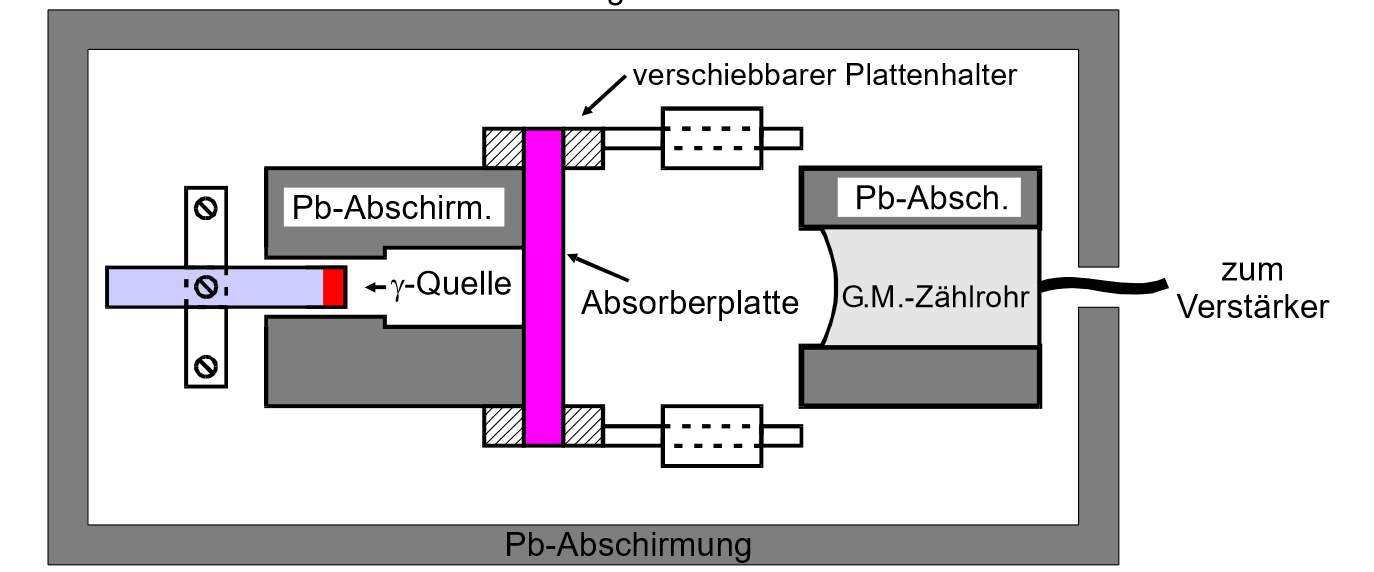
\includegraphics[width=\textwidth]{Bilder/Aufbau.png}
\caption{Abgebildet ist der schematische Aufbau zur Messung der Gamma-Strahlung}
\label{fig:Aufbau}
\end{figure}

Der Versuch wird wie in Abbildung \ref{fig:Aufabu} aufgebaut.
Zuerst wurde die Intensität der Hintergrundstrahlung $I_{Hintergrund}$ über 900 Sekunden gemessen. 
Daraufhin wird eine Eisenplatte zwischen Quelle und Messgerät gestellt und abermals die Intensität $I_E$ gemessen.
Dies wird für bis zu 13 verschiedene Dicken wiederholt, indem weitere Eisenplatten hinzugefügt wurden.
Die Messung wird genau so für Aluminiumplatten durchgeführt. 

\subsection{Absorbtion von Beta-Strahlung}
Für $\beta^{-}$-Strahlung wurde der Aufbau analog zu Abbildung \ref{fig:Aufabu} aufgebaut, nur der Gamma-Strahler wurde durch einen Beta-Strahler ersetzt.
Dann wurden